\section{Aufbau und Durchführung}

In Abbildung \ref{fig:aufbau} ist der Versuchsaufbau dargestellt. Zusätzlich ist der Aufbau rundherum mit Bleiblöcken abgeschirmt. Die $\gamma$-Strahlung
des ${}^{137}Cs$ wird ebenfalls durch einen Bleiblock abgeschirmt, welcher ein kleines Loch hat, damit nur in Richtung des Detektors Strahlung
ausgestrahlt wird. Im Strahlengang wird der Würfel platziert, der vermessen wird. Er ist verschiebbar und drehbar, sodass er entsprechend der verschiedenen
Projektionen justiert werden kann. Als Detektor wird ein Szintillationsdetektor verwendet, dessen Ergebnisse mittels eines Computers ausgelesen werden.
Der Szintillationsdetektor besteht aus einem Szintillator und einem Photomultiplier. Im Szintillator regen die Photonen der $\gamma$-Strahlung Elektronen an,
welche wieder Photonen aussenden. So entstehen mehrere Lichtblitze im Szintillator, deren Anzahl abhängig von der Energie der $\gamma$-Strahlung ist. Diese
Lichtblitze werden vom Photomultiplier in ein elektrisches Signal umgewandelt, dessen Amplitude die Energie der Strahlung angibt und von einem
Multichannelanalyzer histogrammiert wird. Dieses Signal wird vom Analyseprogramm des Computers ausgelesen und aufgetragen.

\begin{figure}
  \centering
  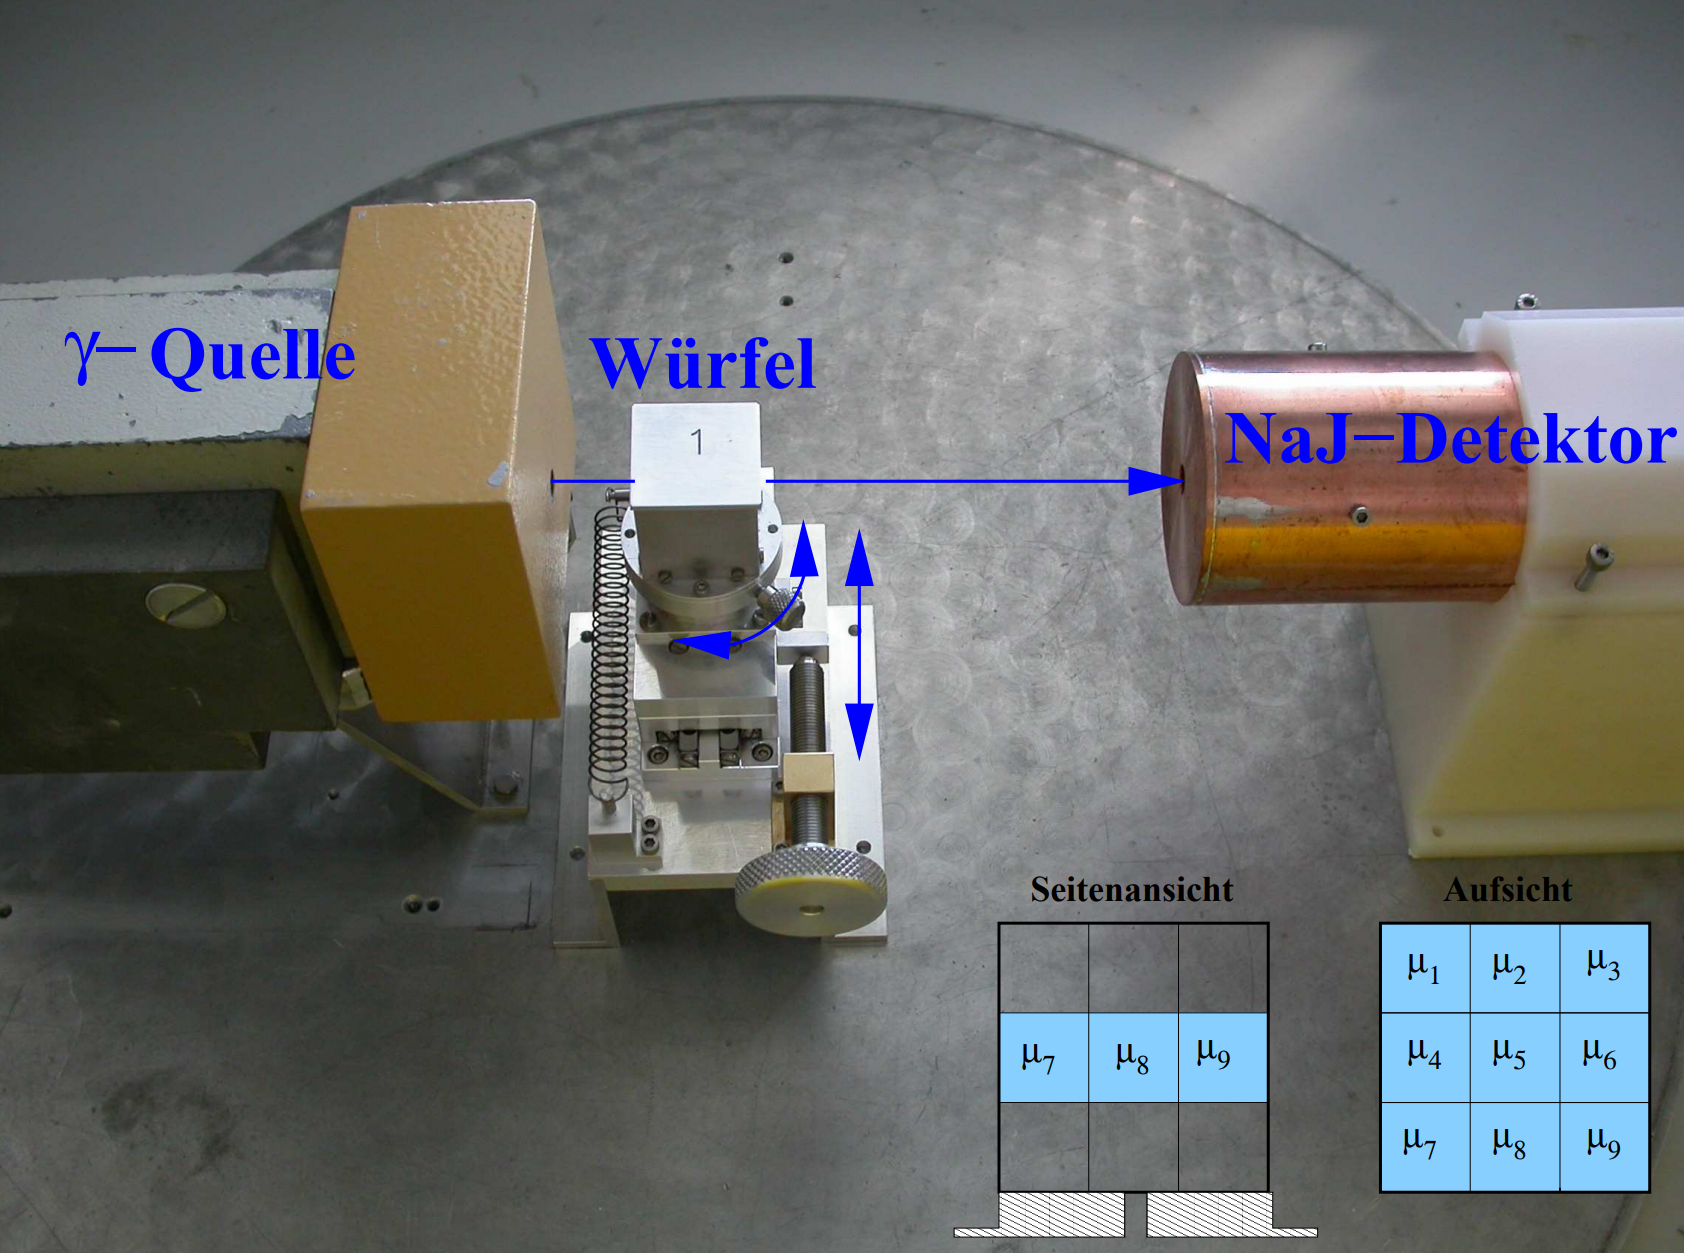
\includegraphics[scale=0.5]{graphics/Aufbau.png}
  \caption{Versuchsaufbau ohne Bleiabschirmung.\cite{anleitung}}
  \label{fig:aufbau}
\end{figure}

Zu Beginn werden vier verschiedene Vergleichsmessungen aufgenommen. Zuerst wird eine Nullmessung des Spektrums der ${}^{137}Cs$-Quelle durchgeführt.
Da der zu vermessende Würfel von einer dünnen Aluminiumhülle umschlossen ist, wird nun eine leere Aluminiumhülle vermessen. Zudem werden ein reiner
Aluminiumwürfel und ein reiner Bleiwürfel vermessen. Mit diesen drei Würfeln werden jeweils 3-4 Messungen durchgeführt. Danach wird Würfel 5 vermessen,
welcher sich aus unbekannten Elementarwürfeln zusammensetzt. Diese Messung wird entsprechend Abbildung \ref{fig:wuerfel} durchgeführt.
